%regulation
\subsection{Introduction}
%~~~~~~~~~~~~~~~~~~~~~~~~~~~~~~~~~~~~~~~~~~~~~~~~~~~~~~~~~~~~
La régulation se trouvant sur l'Arduino Motor a pour objectif de faire avancer le robot afin qu'il suive exactement une trajectoire donnée. Avant de commencer la régulation en tant que telle, il faut se poser quelques questions :

\begin{itemize}
	\item Où veut-on aller ? La consigne est envoyée par l'Arduino Master via l'I\up{2}C;
	\item Comment commander les moteurs afin de faire avancer le robot ? Il suffit d'envoyer une commande appropriée au driver;
	\item Vers où le robot se dirige ? Où est-il par rapport à l'objectif ? Des roues codeuses sont utilisées afin de connaitre la distance parcourue depuis que la consigne a été donnée;
	\item Il y a-t-il un obstacle devant nous ? Des capteurs ultrasons ont la possibilité d'arrêter le robot s'il s'approche trop près d'un obstacle.
\end{itemize}

\paragraph{}
Avec ces informations à disposition, il est possible de faire une régulation. Les points suivants vont détailler la problématique de chaque question, puis proposer une solution de régulation.

\subsection{Consigne et commande des moteurs}
%~~~~~~~~~~~~~~~~~~~~~~~~~~~~~~~~~~~~~~~~~~~~~~~~~~~~~~~~~~~~
\subsubsection{Commande des moteurs}
%~~~~~~~~~~~~~~~~~~~~~~~~~~~~~~~~~~~~~~~~~~~~~~~~~~~~~~~~~~~~
La commande des moteurs se fait par l'intermédiaire du driver. Celui-ci a besoin de deux signaux de commande par moteur :

\begin{itemize}
	\item DIR1 et DIR2, qui définissent le sens dans lequel tourne les moteurs ;
	\item PWM1 et PWM2, qui définissent la vitesse de rotation des moteurs.
\end{itemize}

\paragraph{}
Ces quatre commandes permettent de définir cinq actions possibles pour le robot, ces dernières sont reprise au tableau~\ref{tb:ActionsMoteurs}. On considère le moteur 1 comme étant le moteur de droite et le moteur 2 celui de gauche. 

\begin{table}[!ht]
	\centering
	\begin{tabular}{|l|cc|cc|}
		\hline
		& DIR1 & DIR2 & PWM1 & PWM2 \\
		\hline
		Forward & 1 & 1 & \multicolumn {2}{c|}{Variable} \\
		\hline
		Backward & 0 & 0 & \multicolumn {2}{c|}{Variable} \\
		\hline
		Turn Left & 1 & 0 & \multicolumn {2}{c|}{Variable} \\
		\hline
		Turn Right & 0 & 1 & \multicolumn {2}{c|}{Variable} \\
		\hline
		Stop & \multicolumn {2}{c|}{X} & 0 & 0 \\
		\hline
	\end{tabular}
	\caption{Commandes des moteurs}
	\label{tb:ActionsMoteurs}
\end{table}

\paragraph{}
Au niveau du code, un problème s'est posé pour la réalisation de la PWM. En effet, il existe une manière très simple de créer une PWM en utilisant la fonction \lstinline$analogWrite()$. Cependant la fréquence de la PWM ainsi obtenue était, au maximum, de 1kHz. Pour que le moteur fonctionne correctement, il faut une PWM de fréquence de l'ordre de la dizaine de kHz ou plus. Il a donc fallu trouver une autre manière de créer une PWM à une fréquence plus élevée.

\paragraph{}
La solution à ce problème vient de la librairie \lstinline$"PWM.h"$. Celle-ci permet, entre autre, de changer la valeur de prescaler des timers. On a deux choix pour le faire, soit on utilise la fonction \lstinline$pwmWrite()$ qui a un fonctionnement analogue à \lstinline$analogWrite()$. Soit on va jouer directement sur un timer en particulier en utilisant les fonctions disponible dans la librairie. Le fait qu'on aille jouer sur les prescalers des timers peut être dangereux si on utilise une fonction de base liée au temps (ex: \lstinline$delay()$). On peut se référer à la table~\ref{tb:LienTimerPin} pour voir quel timer est relié à quelle pin afin de ne modifier que ce qui est utile.

\begin{table}[!ht]
	\centering
	\begin{tabular}{|l|c|c|c|c|c|c|}
		\hline
		Timer\# and channel & TIMER3B & TIMER3C & TIMER0B & TIMER3A & TIMER4A & TIMER4B \\
		\hline
		Pin\# & 2 & 3 & 4 & 5 & 6 & 7 \\
		\hline
		\hline
		Timer\# and channel & TIMER4C & TIMER2B & TIMER2A & TIMER1A & TIMER1B & TIMER0A \\
		\hline
		Pin\# & 8 & 9 & 10 & 11 & 12 & 13 \\
		\hline
	\end{tabular}
	\caption{Lien entre les timers et les pins}
	\label{tb:LienTimerPin}
\end{table}

\subsubsection{Consigne}
%~~~~~~~~~~~~~~~~~~~~~~~~~~~~~~~~~~~~~~~~~~~~~~~~~~~~~~~~~~~~
La consigne est donnée par l'Arduino Master sous la forme évoquée au point~\ref{sub:EntreArduinos}. 

\noindent Il y a 12 bits de data qui peuvent être utilisés, soit un nombre de 0 à 1024. Ceux-ci représentent le déplacement que le robot va devoir effectuer. Le déplacement est considéré en nombre d'impulsions reçues provenant des roues codeuses. La régulation interprétera le déplacement afin de fournir les PWM pour commander les moteurs. Il faut se référer au point sur les roues codeuses et au point sur la régulation pour plus d'informations. 

\noindent Une deuxième information donnée est la fonction, elle permet de définir le sens de la marche du robot (DIR1 et DIR2).

\subsection{Roues codeuses}
%~~~~~~~~~~~~~~~~~~~~~~~~~~~~~~~~~~~~~~~~~~~~~~~~~~~~~~~~~~~~
Les roues codeuses sont utilisées pour connaître avec exactitude la distance parcourue en passant outre le glissement\footnote{Glissement: Différence entre le nombre de tours du moteur et le nombre réel de tours de roues parcourus.}. En effet, le glissement que l'on pourrait avoir, par exemple en crissant les pneus au démarrage, nous donnerait une information \textit{fausse} puisque l'information serait \og Nous avons fait 1 tour de roue\fg alors que le robot n'a pas encore bougé.

\subsubsection{L'incrément}
%~~~~~~~~~~~~~~~~~~~~~~~~~~~~~~~~~~~~~~~~~~~~~~~~~~~~~~~~~~~~
Notre travail sur les roues codeuses a été de déterminer le sens de rotation, puis d'incrémenter ou décrémenter un compteur global de façon à avoir le nombre d'impulsions parcourues pour chacune des roues. 

\paragraph{}
Pour détecter le sens de rotation, il suffit de travailler avec des états. En effet, comme montré à la figure~\ref{img:rotary_encoder}, nous sommes en présence de quatre états qui s'enchaîneront d'en un sens ou dans l'autre selon la direction des roues. De plus, l'autre contrainte majeure est le travail des roues codeuses sur des interruptions. En effet, le code dans les interruptions \emph{doit} être le plus \emph{court} possible car il s'exécutera même si une autre action était occupée \textbf{et} il mettra en pause les compteurs (sauf \lstinline$millis()$). 

\subsubsection{Le code}
%~~~~~~~~~~~~~~~~~~~~~~~~~~~~~~~~~~~~~~~~~~~~~~~~~~~~~~~~~~~~
Nous avons donc compressé le code pour qu'il devienne le plus court possible et le plus facile à optimiser pour le compilateur. Ainsi, nous stockons la valeur actuelle de l'état qui a varié dans \textit{stateDroitA} et \textit{stateDroitB}, puis nous incrémentons décrémentons le compteur \textit{compteurDroit}, si l'interruption provient de A, si l'état actuel de A est différent de l'état précédent de B alors nous ajoutons 1 et s'il est le même alors nous retranchons 1. Naturellement la condition est inversée si l'interruption provient de B.

\begin{lstlisting}[language=C++,frame=tblr,keywordstyle=\bfseries]
void DroitA(){
  stateDroitA=digitalRead(19) == HIGH;
  compteurDroit += (stateDroitA != stateDroitB) ? +1 : -1;
}

void DroitB(){
  stateDroitB=digitalRead(18) == HIGH;
  compteurDroit += (stateDroitA == stateDroitB) ? +1 : -1;
}
\end{lstlisting}

\begin{figure}[!ht]
	\centering
	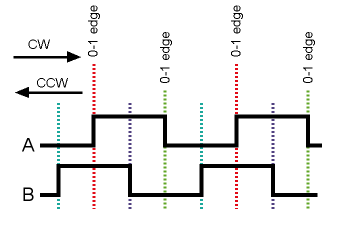
\includegraphics{roues_codeuses.png}
	\caption{Signal des roues codeuses}
	\label{img:rotary_encoder}
\end{figure}

\subsection{Capteurs ultrasons}
%~~~~~~~~~~~~~~~~~~~~~~~~~~~~~~~~~~~~~~~~~~~~~~~~~~~~~~~~~~~~
Dans ce projet, les capteurs ultrasons ne servent qu'à une seule chose, la détection d'obstacle. Il faudra alors mettre plusieurs capteurs tout autours du robot. Le principe de ces capteurs est assez simple. Il faut d'abord envoyer une impulsion et ensuite attendre qu'elle revienne. Le temps entre l'envoi et la réception de l'impulsion représente la distance parcourue, il faut donc le convertir afin d'avoir une distance en mètre. 

\paragraph{}
Pour utiliser les capteurs avec l'Arduino Moteur, il faut pouvoir compter le temps de parcours de l'onde. Il existe une fonction qui rend cela assez simple, \lstinline$pulseIn()$. Malheureusement, cette fonction bloque l'Arduino le temps que l'impulsion revienne à moins que le timeout (1ms) soit dépassé. Cela rend la campagne de mesure de tout les capteurs extrêmement longue. En effet, on ne peut pas gérer les interruptions\footnote{Les interruptions sont utilisées pour la communication I\up{2}C ainsi que par les roues codeuses.} pendant tout ce temps. Il a fallu trouver une autre méthode pour utiliser de manière optimisée les capteurs.

\paragraph{}
Cette deuxième méthode se base sur l'utilisation de la librairie \lstinline$"NewPing.h"$. Cette dernière à l'avantage de ne pas bloquer l'Arduino lors de l'attente du signal de retour car elle utilise un timer au lieu de \lstinline$pulseIn()$. On peut donc continuer à recevoir des interruptions pendant que le timer compte de son côté. L'utilisation d'un timer a cependant un inconvénient. Il faut faire en sorte qu'on n'utilise pas le même timer dans le reste du code et que la modification de son prescaler n'entraine pas de dysfonctionnement \footnote{Notamment pour la génération des PWM.}. Les pins à éviter sont les pins 9 et 10. Lors des tests effectués, aucune anomalie n'a été détectée.

\subsection{Régulation}
%~~~~~~~~~~~~~~~~~~~~~~~~~~~~~~~~~~~~~~~~~~~~~~~~~~~~~~~~~~~~
La régulation que nous avons réalisée est en fait deux régulateurs entremêlés. Un régulateur proportionnel pour s'assurer que l'on a fait 1000 tics par exemple et un régulateur intégrateur pour éviter d'avoir une erreur entre les deux roues qui fera tourner le robot.

\paragraph{}
Pour avancer, nous donnons une consigne \textit{Deplacement} de x impulsions, pour reculer, nous donnons une consigne \textit{Deplacement} de -x impulsions, et enfin, pour tourner, nous laissons la consigne \textit{Deplacement} à 0 et nous donnons une consigne de \textit{Glissement}.

\noindent De plus, si le glissement est non nul, alors la PWM du moteur de gauche sera différente de la PWM du moteur de droite.

\begin{figure}[!ht]
	\centering
	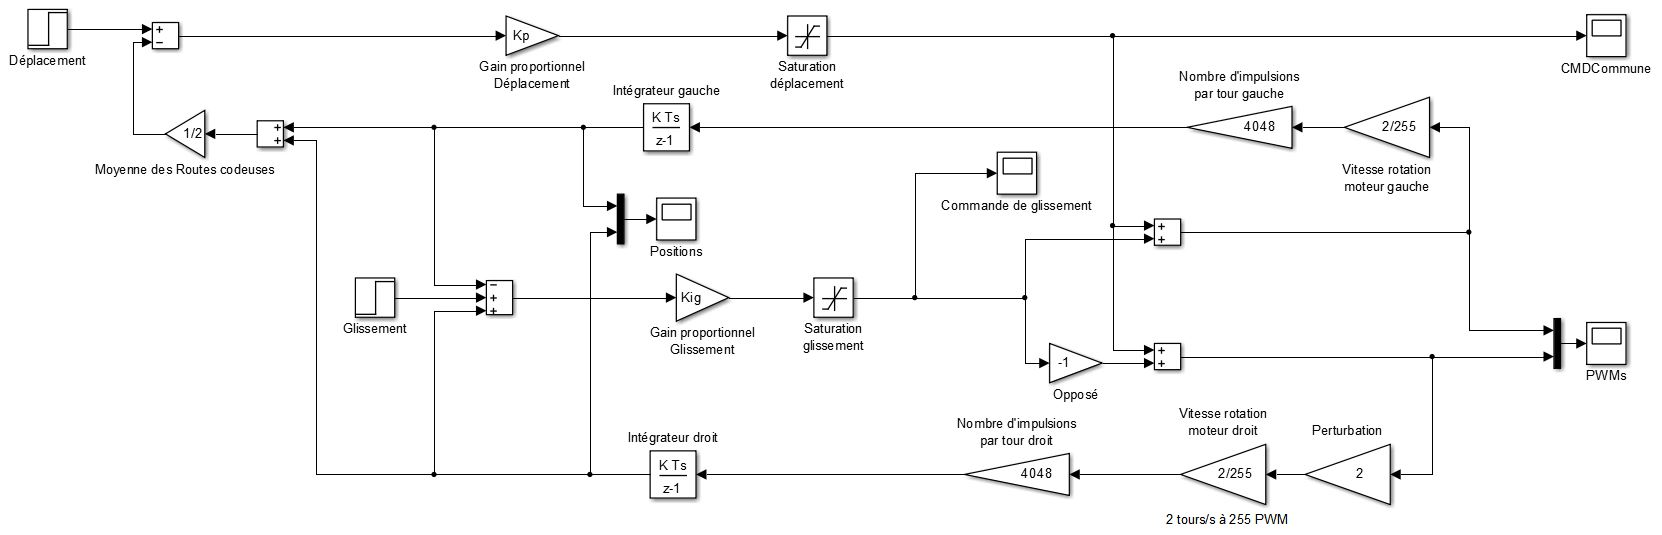
\includegraphics[width=15cm]{simulink.jpg}
	\caption{Schéma bloc de la régulation des moteurs}
	\label{img:simulink}
\end{figure}

\subsubsection{Coefficients Kp et Kig}
%~~~~~~~~~~~~~~~~~~~~~~~~~~~~~~~~~~~~~~~~~~~~~~~~~~~~~~~~~~~~
Les coefficients Kp et Kig permettent de gérer la régulation. Kp multiplie la consigne pour obtenir la PWM et limite la vitesse quand on se rapproche de l'objectif et Kig multiplie la différence entre les deux roues, soit l'intégrale de l'erreur, la somme de l'erreur, pour la réguler et la remettre à 0.

\noindent Le coefficient Kp a été déterminé en choisissant Kp tel que la commande décroisse à partir de 4048. (Donc la commande vaut 255 à 4048 et 0 à 0.) $$Kp = 0.01$$ nous semble bien fonctionner sur Simulink

\noindent Le coefficient Kig a été déterminé en choisissant Kig tel que la commande soit de 50 pour 4048 tics. (Donc il y a une réaction à partir de 40 tics.) $$Kig = 0.005$$ nous semble bien fonctionner sur Simulink

\subsubsection{Essais simulink}
Pour les tests de régulation, nous avons d'abord vérifié que tout marchait bien dans les conditions normales. Malheureusement, tout allait bien et nous avons donc inclus des perturbations en tout genre. Pour les exemples ci-dessous, nous avons choisi un moteur droit qui était deux fois plus rapide que le moteur gauche. Nous sollicitons donc beaucoup le régulateur de glissement.\\

\begin{center}
\textbf{Test en déplacement}
\end{center}

\begin{figure}[ht!]
    \begin{minipage}[b]{0.4\linewidth}
        \centering 
        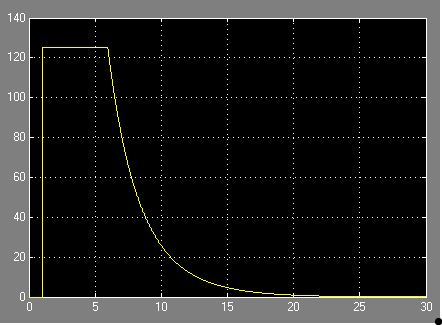
\includegraphics[width=6cm]{deplCMD.jpg}
        \caption{Position des deux roues}
%\caption sert à inserer une légende
    \end{minipage}\hfill
    \begin{minipage}[b]{0.48\linewidth}
        \centering 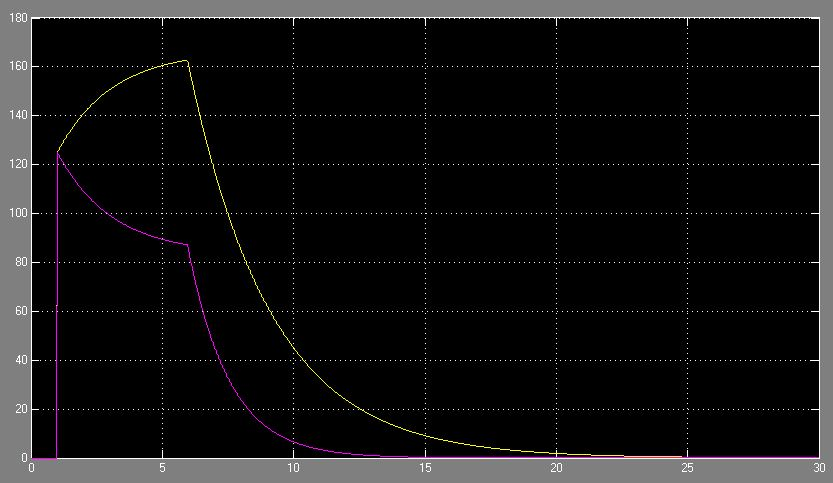
\includegraphics[width=6cm]{deplCMDindiv.JPG}
        \caption{Commande de chacun des moteurs}
    \end{minipage}
\end{figure}

Comme nous pouvons le voir, la commande sera différente grâce au feedback des roues codeuses. De plus, la commande décroit lorsque l'on se rapproche de l'objectif.
\hfill \\

\begin{center}
\textbf{Test en glissement (commande de 25k)}
\end{center}

\begin{figure}[ht!]
    \begin{minipage}[b]{0.4\linewidth}
        \centering 
        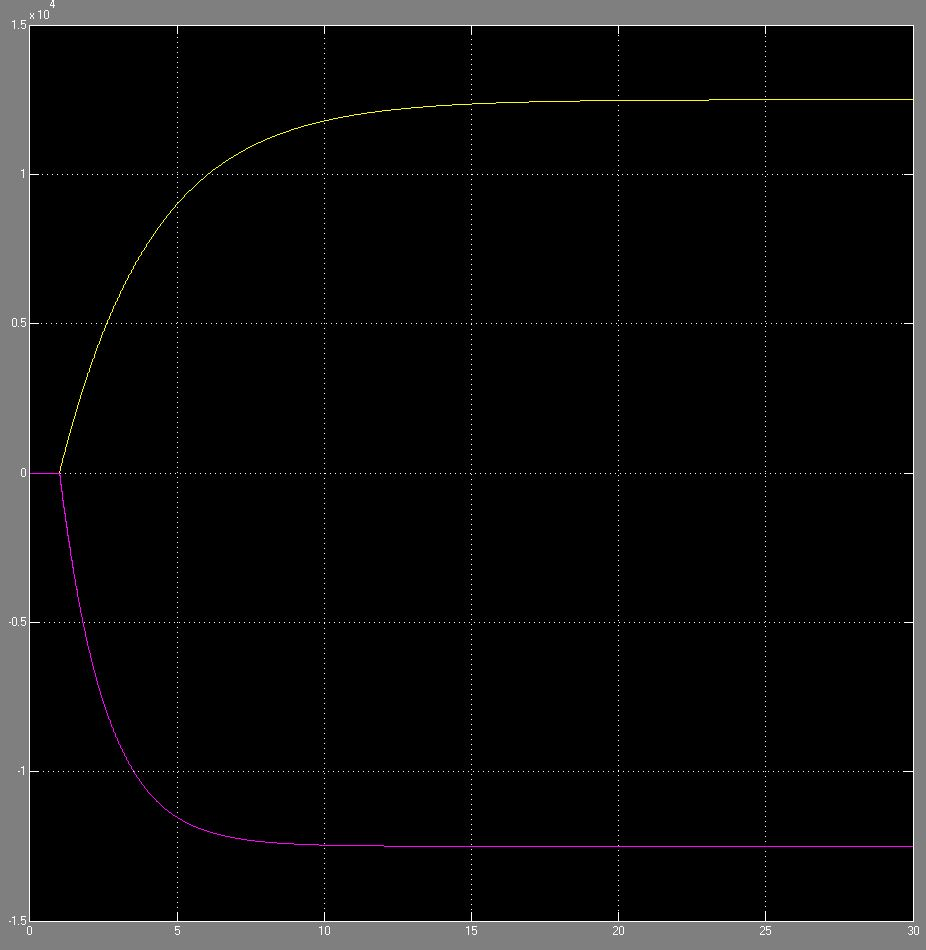
\includegraphics[width=6cm]{glisPos.JPG}
        \caption{Position des deux roues}
%\caption sert à inserer une légende
    \end{minipage}\hfill
    \begin{minipage}[b]{0.48\linewidth}
        \centering 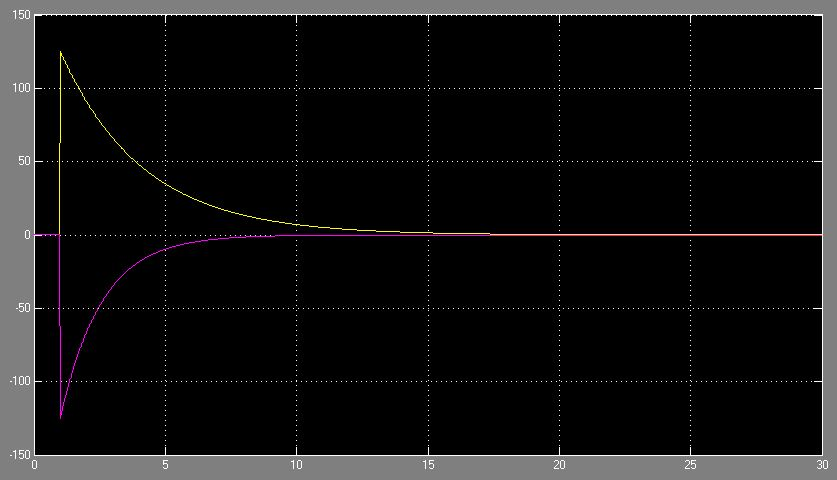
\includegraphics[width=6cm]{glisCMD.JPG}
        \caption{Commande de chacun des moteurs}
    \end{minipage}
\end{figure}

Nous pouvons remarquer dans ces deux graphes que bien que le moteur droit tourne deux fois plus vite que le gauche, le déplacement parcouru par chacun est équivalent.
